\section{Background}
\label{sec:background}
This section briefly recalls both fundamentals of page-table-based address translation in
general-puspose OS kernels, 
high-level background on separation logics and the \iris~\cite{jung2018iris} framework
we build on,
and some material on modal logic that informs our development.

\subsection{Machine Model}
\label{sec:backgroundonmachinemodel}

In typical system configurations, all memory addresses seen by programs running on modern computers are \emph{virtualized}: the address observed by a running
program generally will not correspond directly to the physical location in memory, and may not even correspond to a physical location that \emph{exists} 
in the machine. Instead, these \emph{virtual} addresses are translated to \emph{physical} addresses that correspond directly to locations in RAM. On most 
modern architectures, this translation is performed through cooperation of the hardware and OS kernel: while executing an instruction that dereferences a 
(virtual) address, the CPU's \emph{memory management unit} (\textsc{MMU}) hardware performs \emph{address translation},
resulting in a physical address used to access the cache\footnote{Technically, for performance reasons most caches are indexed with parts of the virtual 
address, but tagged with the physical data addresses, so cache lookups and address translations can proceed in parallel.} and/or memory-bus.

\begin{figure}
    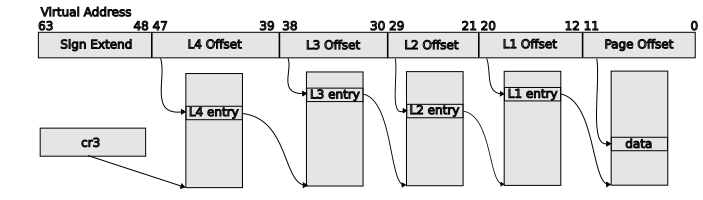
\includegraphics[width=\columnwidth]{pagetables2.png}
    \vspace{-2.5em}
    \caption{x86-64 page table lookups.}
    \label{fig:pagetables}
    \vspace{-1em}
\end{figure}

On the x86-64 architecture, the \textsc{MMU}'s address translation uses a sparse hierarchical set of tables:
\emph{page tables} (referring to pages of memory). As Figure \ref{fig:pagetables} (based on Figure 5-17 of the 
AMD64 architecture manual~\cite{amd64_manual_vol2}\footnote{While x86 up through its 32-bit incarnation were due to Intel,
the x86-64 architecture as a 64-bit extension to x86 was originally due to AMD. As a result, it is sometimes also referred to as the \texttt{amd64} architecture.}) shows, 
address translation proceeds by repeatedly taking designated slices of the virtual address and indexing into a table.
The final lookup in the page tables gives the base physical address of a 4KB page of physical memory, to which the low-order
bits of the accessed virtual address are added to determine the actual physical address retrieved. 
On x86-64, standard configurations use 4 levels of page tables, labelled levels 4 through 1, with lookups in the level 
1 page table resulting in the actual page of physical memory holding the requested data, and the low-order 12 bits 
being used to index into this page.\footnote{Technically levels 1--3 have explicit historical names,
but for brevity and consistency, we simply number them, in keeping with the newer 5th level.
Our formalization
only deals with 4-level page tables, but is straightforwardly extensible to 5.}  
The translation process or algorithm is sometimes referred to as a \emph{page-table walk}. 
While Figure \ref{fig:pagetables} and most of our constants (how many levels, which virtual address bits index which
table levels) are specific to the x86-64 architecture, ARMv8 (a.k.a.\ 
\texttt{aarch64}), RISC-V, and PowerPC use similar hierarchical page tables for address translation.
RISC-V's \texttt{sv48} paging configuration~\cite[\S 4.5]{riscv-privileged} and AArch64's 4-level paging configuration
both split 64-bit virtual addresses at the same points to index into the respective tables, so most of what follows
is equally applicable to those architectures (the only difference is that page table entries place control bits of write access, etc.,
in different orders).

The entries of each table are 64 bits wide, but each points to a physical address aligned to 4KB (4096 byte) boundaries, which leaves 12 bits to spare to 
control a validity bit (called the \emph{present} bit), a read-write bit (which permits write access through the entry if and only if it is set), 
and a range of additional bits which can be used to control caching, write-through, and more. This paper will only consider the present bit (0).

The page tables are managed by the OS, typically by a \emph{virtual memory manager} (VMM).\footnote{Not to be confused with Virtual 
Machine Monitor. We focus on non-hypervisor scenarios, but hardware virtualization extensions for both 
x86-64 and ARM make use of an additional set of page tables translating what a \emph{guest} considers to be its 
(virtualized) physical memory to actual physical memory. Our contributions should offer value in this scenario as well.}
Typically each process has its own 
page table, which the OS registers with the CPU by storing the (page-aligned)
physical address of the root of the page table treethe start of the L4 table) in a 
specific register (\texttt{cr3}) as part of switching to a new process. 
Using different mappings, which map only disjoint portions of physical memory (with some exceptions in the next section) 
is how the OS ensures memory isolation between processes.

If an instruction is executed that accesses a virtual address that either has no mapping, or does not have a mapping permitting 
the kind of access that was performed (e.g., the instruction was a memory write, but the relevant address range was marked read-only in
the relevant page table entry), the hardware triggers a \emph{page fault}, transferring control to a \emph{page fault handler} registered 
with the hardware by the OS, allowing it to take corrective action.
If no mapping was supposed to exist, this is a program bug (e.g., dereferencing virtual address 0 / NULL)
and the faulting program should be terminated. But this can also be used for
specialized functionality and optimizations, such as \emph{paging} (saving room in physical RAM and deferring
unnecessary IO by only reading program code from disk when it is accessed, or even swapping memory that has not
recently been accessed to disk, to read back in when a page fault indicates access).

The key pieces of VMM functionality are
adding a new page mapping (whether the mapped page contains zeros, file data, or swap data), and removing an existing 
page mapping.
While this initially sounds like relatively modest functionality whose implementation may be complicated by hardware 
subtleties, correctness of even these basic operations are actually quite intrictate.
Notably, updates to the page tables are performed as writes to memory --- \emph{which are themselves subject to address translation},
and finding the correct page table to update requires converting between physical and virtual addresses.
In the case of changing the mappings for the currently-active set of page tables, 
\emph{the OS kernel is modifying the tables involved in its
own access of the tables}.

Virtual memory concerns propagate to the OS scheduler, which deals with multiple 
address spaces, so must keep track of which virtual addresses are valid (and in what way) in which address spaces. 
Some virtual addresses are valid in only a single address space (e.g., a code address for a particular usermode 
process), while others are valid in all address spaces (e.g., kernel data structure pointers). 
The VMM must maintain some of these assumptions on behalf of the rest of the kernel, for example by guaranteeing that 
a certain range of virtual addresses (corresponding to the kernel's code and data) are valid in every address space.

\paragraph{Out of Scope: Translation Lookaside Buffers (TLBs)}
CPUs with MMUs typically have an additional \emph{translation lookaside buffer}
(TLB), to cache the (successful) results of page table walks, rather than transforming every virtual
memory access into 5 physical accesses. 
Any time a virtual address that was accessible becomes inaccessible (or has downgraded permissions),
the TLB (or at least entries in affected virtual address ranges) should be flushed.
In most kernels, this occurs in only a few well-known places, which is why existing verified kernels
\textsc{seL4}~\cite{Klein2009seL4,seL4TOCS} and \textsc{CertiKOS}~\cite{gu15,gu2016certikos} currently
trust that TLB flushes are handled correctly rather than actually modeling TLB hardware and verifying.
Eventual verification of TLB handling is a worthwhile long-term goal, but it is a challenging pursuit in its
own right. Based on others' early progress on verifying TLB operations in isolation~\cite{syeda2020formal}, we expect
it to be possible to combine this paper's insights with that support. 
Section \ref{sec:relwork} elaborates briefly on the challenges involved.
Even without TLB modeling,
our logic already enables verification of virtual memory management functionality that prior verified kernel work
either trusts completely (\textsc{seL4}, \textsc{CertiKOS}) or is incapable of reasoning about.
% Appendix \ref{apdx:tlb} gives more details on the challenges involved for the interested reader.
\looseness=-1

% \subsection{Virtual Memory Managers}
% \label{sec:backgroundonvmm}
% Most OS kernels have a component called a \emph{Virtual Memory Manager} (VMM)
% which is responsible for setting up page table mappings and for taking action when a page fault occurs. Often, a page 
% fault indicates a bug in a program --- for example, a null pointer dereference crashes a program not because the hardware
%  designates it an error, but because most OSes refuse to map the first 4K worth of virtual addresses, so dereferencing 
% \texttt{NULL} results in a page fault. In such cases, the OS will terminate the program.

% In other cases the OS uses page faults to implement specialized functionality and optimizations. A key example of this is 
% (confusingly) called \emph{paging}: saving room in physical RAM and avoiding unnecessary IO 
% by waiting until memory addresses for code are accessed 
% before copying them to RAM (in particular, saving process startup time); 
% or copying memory that has not recently been accessed to disk 
% (i.e., in a \emph{swap} file or partition) and marking those page table entries invalid so a future page fault will give 
% the OS the chance to copy the relevant data back into memory when the program tries to access it again.


% \todo[inline]{Colin says: we should chat about the paragraph below. We don't want to advertise too many
% challenges of VMM verification that we don't actually solve (or rather, we'd push them to the and of the paper
% as future work). But some of these I think we could split the difference with, for example by defining
% a variant of virtual-pointsto that allowed virtual address aliasing, but not actually verifying any code examples
% with it (just showing it's compatible with our approach).
% }
% For one, virtual addresses may \emph{alias} when more than one is mapped to the same physical memory. 
% This can occur when a process requests it (e.g., via \texttt{mmap} or \texttt{shm\_open} on UNIX-style kernels). 
% It also occurs automatically in most general-purpose kernels: while for normal programs the OS uses the MMU to isolate 
% and abstract physical memory, the kernel's own functionality is often easier to implement if the kernel can directly 
% access memory given its physical address, for example when interacting with hardware devices. For this reason, most 
% kernels contain an \emph{identity map} of all physical memory in a machine. 
% \todo[inline]{We should try defining an identity map on a whiteboard and see what breaks. If it's feasible we should
% tweak and get a definition in the paper. If not, we should cut the identity map discussion.}
% In some cases this is a literal identity map, 
% where for every virtual address $p$, interpreting $p$ as a virtual address instead will map back to $p$ as a physical 
% address. In other cases there is an offset involved, where to access physical address $p$ the kernel can access virtual
%  address $p+\mathit{offset}$. This identity map saves the kernel the performance cost of having to continually add and
%  remove transient mappings simply to briefly access a specific physical memory region. But this coexists with additional
%  virtual addresses (those used by most kernel code and data structures), in a form of virtual address aliasing. Note 
% that virtual address aliasing is both prevalent in general-purpose kernels, and violates the core assumption of most 
% memory models assumed by verified compilers like CompCert, which assume no virtual address aliasing.

% \todo[inline]{Colin says: Again, let's chat about the next paragraph. This might be another where we can
% split the difference on extension by defining something and proving a $\ast-\ast$ kind of result for sharing
% page table fragments, rather than actually proving any new code. I'm less sure about this one, though.
% }
% Another complicating factor is that portions of page tables can be shared, i.e., trees of page tables can overlap and
% become forests. 
% One common way this used to happen was for one subtree of page tables to map the kernel if linked in appropriately to 
% a higher-level page table, and then to reuse that kernel mapping portion in every process's page tables. This was mostly 
% phased out in the wake of Spectre, but remains relevant on correctly-implemented hardware.

\subsection{Separation Logic}
\label{sec:seplogic}
% \todo{Colin says: I added this b/c prior systems reviewers wanted more verification background...
% not sure how I feel about it}
Separation logic~\cite{reynolds02} is a descendant of classic Hoare logic~\cite{hoare69},
where in addition to pre- and postcondition assertions, assertions themselves pick up a
\emph{separating conjunction} operator $\ast$, such that an assertion $A\ast B$ means $A$ and $B$ are true
of disjoint pieces of state. This allows for local reasoning about updates, because it articulates
that updates to the state backing $A$ do not affect the truth of $B$. This is classically demonstrated
through the \emph{points-to} assertion: $l\mapsto v$ asserts that the memory cell at address $l$ holds value $v$:
knowing $x\mapsto 3\ast y\mapsto 4$ and writing through $x$ means information about $y$ is preserved:
$\{x\mapsto 3\ast P\}\;x\mathrel{:=}5\;\{x\mapsto 5 \ast P\}$ can be derived for any $P$.

We build on the \iris~\cite{jung2018iris} separation logic framework,
an abstract separation logic embedded in Rocq, which is useful for both metatheoretical work
and interactive correctness proofs using the logic. Given an operational
semantics structured a certain way (in our case, semantics for
a fragment of x86-64 assembly including address translation),
if a small number of ``glue'' lemmas are proven, \iris
provides a ready-made separation logic with a number of advanced features, including
higher-order ghost state and impredicative invariants, for no additional work.

We suppress many details of \iris assertions for brevity, but briefly note
a few recurring details used heavily in \iris but not necessarily in traditional
separation logics.
Because \iris is an embedded framework in \rocq, proofs in \iris-derived
logics (including ours) often encapsulate raw \rocq assertions: $\ulcorner P \urcorner$ is an embedding
of the \rocq assertion $P$ into an \iris assertion (used for things like equality and other
general pure logical assertions), similar to prior \rocq-embedded program logics~\cite{Chlipala2013Bedrock}. Newly-defined \iris assertions are in fact
\rocq terms of a particular type, rather than being drawn from a fixed vocabulary.
We introduce other details as they arise.

\iris includes two forms of implication. The magic wand operator $\wand$ is an affine implication:
$A\wand B$ describes a resource which, if combined with a resource satisfying $A$, will satisfy $B$.
Notably, this implication involves no changes to ghost state. \iris, building on the Views framework~\cite{Dinsdale-Young2013Views},
also includes a \emph{view shift} operator $\vs$ which models updates to ghost state: $A \vs B$
means resources satisfying $A$ may be transformed into resources satisfying $B$, intuitively by updating only ghost state.\footnote{\iris
experts may note that this is \emph{technically} mildly misleading given how \iris's update modalities and weakest precondition
are defined, but
this is adequate intuition for non-experts in \iris to follow their use.
}
\looseness=-1

% Of particular interest to us, \iris's machinery is largely agnostic to the particular choice of
% \emph{resource algebra}\footnote{A modern descendant of the venerable partial commutative monoid used
% to abstractly model earlier separation logics~\cite{calcagno2007local}, 
% with additions to support the step-indexing required to solve the recursive domain equations
% that arise with higher-order ghost state and impredicativity~\cite{birkedal2011step,hobor2010theory}.
% }
% used to give algebraic semantics to the connectives of the assertion language.
% This means we can drop in an alternative model that naturally supports working with respect to
% a locally-fixed context, like an address space.

% Also relevant is that \textsc{Iris} naturally decomposes the traditional Hoare triple $\{P\}\;C\;\{Q\}$
% into the precondition implying the weakest precondition of the program with respect to the postcondition ---
% $P \wand \textsf{wp}\;C\;\{v\ldotp Q\}$.\footnote{An idea with long history~\cite{pratt1976semantical}.}
% This is a natural fit for assembly-level verification, where the \emph{Hoare double}

An important limitation here is that to date, every separation logic
has assumed that all pointer addresses are meant for use in a single address space, which avoided the
problem of tracking that certain points-to assertions are true only for certain address spaces, but not others.

\subsection{Modal Logic}
\label{sec:backgroundonmodallogic}
The problem of needing to keep track of things being true in some contexts and not in others is hardly unique to virtual 
memory management, and is the general insight behind most flavors of modal logic, which use
unary operators to express that a logical claim $P$ is \emph{contingently} true 
in certain other circumstances, such as in other times~\cite{pnueli1977temporal} or places~\cite{murphy2008type,gordon2019modal}.

%   A unifying concept across any modality is that they behave as applicative functors, 
% typically satisfying (directly, or as a derived law, depending on the modality):
% \[ (P\rightarrow Q) \rightarrow M(P) \rightarrow M(Q)\]
% %\todo[inline]{Ismail, I think this means we have pure intro, $\square P \mathrel{-\ast} [r](\square P)$ if I'm using the right symbol for pure assertions }
% %\todo[inline,color=red]{The above todo comment isn't quite right.
% %Purity is about being able to duplicate. You had defined another typeclass/property-of-assertions that meant it didn't
% %care what address space it was in (like physical pointstos). That's orthogonal to purity.
% %}
% Many modalities, so-called \emph{normal} modalities also possess introduction rules of the form $P\rightarrow M(P)$, 
% the classic example being that if $P$ is true, then $P$ is \emph{necessarily} true with the contingency picked up.%($\square P$).

Of particular interest for reasoning about virtual memory are modalities that permit \emph{naming} the alternate 
circumstances, prominently \emph{hybrid} modal logics~\cite{blackburn1995hybrid,areces2001hybrid}, which come equipped 
with assertions of the form $[\ell](P)$ indicating that $P$ is true in the specific alternate circumstance (Kripke world)
 named by the \emph{nominal} $\ell$. Note that a distinctive property of hybrid logics is that, rather than hiding
the points at which a modal assertion is evaluated inside the modality's definition, the choice of what world a modalized
assertion should be true in is chosen \emph{in the assertion itself}. This allows assertions to talk about not simply whether some other assertion
is true in some possible future or past world related in a fixed way to the current world, but to talk about \emph{arbitrary}
other worlds. This explicit naming of alternate worlds increases the power of modal logics~\cite{blackburn1995hybrid}, and is actually
necessary for completeness in classical separation logics~\cite{brotherston2014parametric}.
%   A key distinguishing feature of
% hybrid logic is that the logic itself does not fix the set of modalities, but is defined relative to any set of sensible worlds.

For our purposes, these are natural candidates to adapt for virtual memory management. We can reinterpret the notion of 
naming an alternate world slightly more loosely, and instead name \emph{address spaces} by the physical address of the 
page table root, since these structures are the physical representations of page tables. Thus in this paper we develop 
the notion that we can represent contingent truth of an assertion via $[r](P)$ indicating that $P$ holds in the address 
space rooted at physical address $r$. Because OS kernels create and destroy address spaces, it is sensible to use
a hybrid-style logic that is not specialized to a fixed set of modalities, but this introduces
some subtleties from the fact that the existence of certain modalities (address spaces) can change.

% The typical hybrid modality introduction rule, that $P$ and $\ell$ (indicating the current world is $\ell$) imply 
% $[\ell](P)$, has a natural analogue: knowing $P$ and that the current address space is $r$ (i.e., that $r$ is the 
% current \texttt{cr3} value) suggests a way to construct $[r](P)$. 
% We identify an assertion as \emph{contextual} if its validity depends on the choice of address space. Used outside an explicit
% modality, the truth of this assertion depends on the current \texttt{cr3} value. Used under an explicit address space
% modality, its truth depends on both the modality-chosen address space and associated physical resources.
% \begin{itemize}
%   \item as a \textit{contextual} fact if its validity depends on \texttt{cr3} when it is outside the modality (i.e. modal context), and made 
%   \texttt{cr3} independent as a part of custom-tailored modal logic for virtual-memory: a truth representing a virtual-memory addressing depends
%    \texttt{cr3} due to address-translation operation, is dependent on \texttt{cr3} in the ambient-logic (e.g. separation-logic),
%     and is made \textit{independent} of the facts related to \texttt{cr3} by being introduced into the modal context under the assumption that
%     it exhibits the knowledge on its validity with respect to \texttt{cr3} in the ambient logic.
%   \item as a \textit{pure} fact as long as it does not \textit{necessarily} depend on any fact related to \texttt{cr3}: a truth representing a raw physical memory addressing, unlike virtual-address translation, does not need the \textit{knowledge} of \texttt{cr3}, therefore it can be introduce into the modal context as a pure fact
% \end{itemize}

Interaction of hybrid modalities and substructural reasoning is relatively unexplored (see Section \ref{sec:relwork}).
% A relatively under-explored space of modal logics is the interaction of modal and substructural logics, 
% in particular hybrid-style modalities in substructural logics, which has seen only minimal exploration~\cite{dovsen1992modal,restall1993modalities,d1997grafting,kamide2002kripke,licata2017fibrational} and no prior 
% application. 
Our development atop \iris~\cite{jung2018iris} needs to explore some additional subtleties 
that arise where the modality itself may entail ownership of resources, 
as well as interactions between our hybrid-style 
modality and substructural rules.  
% For example, Iris contains a number of modalities that distribute over separating 
% conjunction, or for which resources can freely move into the modality 
% (e.g., $\blacktriangleright(P)\ast Q \wand \blacktriangleright(P\ast Q)$). In our setting some of these rules 
% apply while others do not. For example, 
% In our setting, an assertion that involves no modalities is interpreted as 
% holding in the current (active-on-the-CPU) address space, so clearly cannot move into arbitrary other address spaces,
% while address-space-relative assertions 
% --- unless guarded by another address space modality.
Some prior \iris-based work~\cite{dang2019rustbelt,dang2022compass} has constructed derived modalities in the style we propose, indexed
by thread IDs. However in that setting, the intepretation of those modalities was fully fixed ahead of time (to refer to essentially buffers in operationalized versions of C11
concurrency). In this setting, while our modalities will be indexed by page table roots, it is possible to modify the address translation for an address
space with root $r$ --- thus changing the interpretation of a modality, and even whether a modality is valid --- \emph{while assertions with that modality are active}.
%
%
%Work on modal logic extends back for decades with many widely-varied variations; we discuss here only the pieces most relevant to our work.
%Broadly speaking modal logics incorporate \emph{modal operators}, which take as arguments a proposition expected to be true in another time~\cite{pnueli1977temporal}, place~\cite{gordon2019modal}\todo{other cites}, or circumstance~\cite{hintikka1962knowledge,halpern1985guide}, and result in a proposition true in the \emph{current} time, place, or circumstance at which the truth of the use of the modal operator is being evaluated. Classic examples include modal necessity $\square P$ describing that $P$ is \emph{necessarily} true, $\mathsf{G}~P$ meaning $P$ is true \emph{globally} (i.e., forever from this time onwards), or $K_i(P)$ describing that a particular participant $i$ \emph{knows} that $P$ is true. The latter is an example of of \emph{multimodal} logic, where there is an indexed family of modalities (modal operators) parameterized by some dimension of interest (there, participants).
%A closely related variant of multimodal logic is \emph{dynamic logic}~\cite{pratt1976semantical}, a logic of weakest preconditions~\cite{dijkstra-75} which works with modalities of the form $[p](P)$, which states that \emph{in the current program state}, \emph{if} program $p$ is run then afterwards $P$ will hold (modulo non-termination).
%This same idea is used to encode Hoare triples in the Iris program logic~\cite{krebbers2017essence}, using the same encoding as in Pratt's original presentation, where a Hoare triple $\{P\}C\{Q\}$ is encoded as $P\rightarrow[C](Q)$. Unlike classic work on dynamic logic~\cite{harel2000dynamic}, Iris applies these ideas in a \emph{substructural} setting (separation logic) where distributivity laws over substructural connectives must be considered. For both the dynamic modality and the later modality $\blacktriangleright$ used for guarded recursive predicates, these modalities satisfy axioms of the form $M(P)\ast Q\vdash M(P\ast Q)$, but not the reverse.
%Iris is not the first combination of modal and substructural logic~\cite{dovsen1992modal,restall1993modalities,d1997grafting,kamide2002kripke,licata2017fibrational}, but is certainly the most heavily tested.
%A hallmark of a unary logical operator $M$ being a modality is if $M$ satisfies an property akin to $(\upvarphi\rightarrow\psi)\rightarrow M(\upvarphi)\rightarrow\psi$, which roughly states that modus ponens holds under the modality.\footnote{Afficionados of modal logic will note that this property is not quite Axiom K (which requires the initial implication to also hold under $M$), but follows from K and a necessitation rule $\upvarphi\rightarrow M(\upvarphi)$. Non-necessitive modalities typically satisfy the weaker property we call out above.}
%Another pillar of our work is hybrid logic, a branch of modal logic with \emph{names} (called \emph{nominals} for states in Kripke models~\cite{blackburn1995hybrid,goranko1996hierarchies,areces2001hybrid,gargov1993modal}, in contrast to the typical flavor of modality which refers to an \emph{unspecified} (in the assertion) set of alternative circumstances. 
%
%Our work draws on ideas from hybrid modal logics, applied in the context of Iris's higher-order separation logic~\cite{jung2018iris}. We define our modalities and prove their rules directly within Iris, so there is no model-theoretic novelty in our work. Instead, we show that targeted use of modalities combining the ideas of \emph{named resources} with the power of substructural reasoning enable clear specification of general reasoning principles for data structures. Along the way we take advantage of the fact that modalities need not be injections between the \emph{same} logics, but in fact the propositions that modal operators contextualize can come from \emph{other} logics; in our case we exploit the fact that Iris itself is parameterized by a choice of step-indexed~\cite{ahmed-appel-virga-02} \textsf{BI}-algebra~\cite{ohearn1999bunched} to allow convenient specifications in embedded data-structure-relative logics.
